\section{Graficzny interfejs użytkownika}

\subsection{Opis dostępnych funkcji}
W ramach niniejszej pracy zaimplementowany został graficzny interfejs użytkownika. Umożliwia on obsługę większości opisanych we wcześniejszych sekcjach funkcji. Pozwala na korzystanie z opracowanego oprogramowania bez znajomości języka Python. Uruchamianie interfejsu odbywa sie z poziomu IDE, w tym przypadku z Pycharma. W drzewie projektu należy odnaleźć katalog o nazwie $GUI$, następnie plik $api\_main.py$. Rysunek \ref{fig:gui_tu_jest}

\begin{figure}[h]
\centering
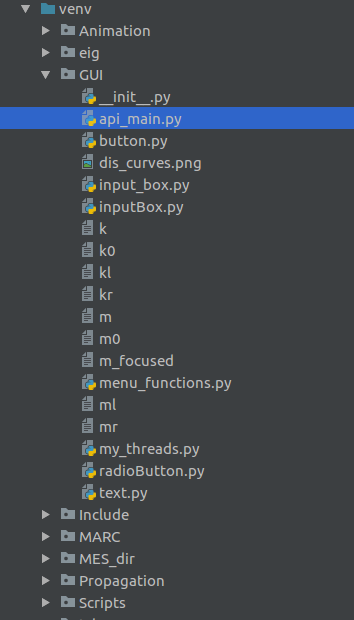
\includegraphics[width=8cm]{Zdjecia/5/kasia/gui_drzewo}
\caption{Położenie $api\_main.py$ w drzewie projektu}
\label{fig:gui_tu_jest}
\end{figure}

Po uruchomieniu programu $api\_main.py$ wyświetlany zostaje graficzny interfejs. Rysunek \ref{fig:gui1} przedstawia wygląd interfejsu zaraz po uruchomieniu.

\begin{figure}[h]
\centering
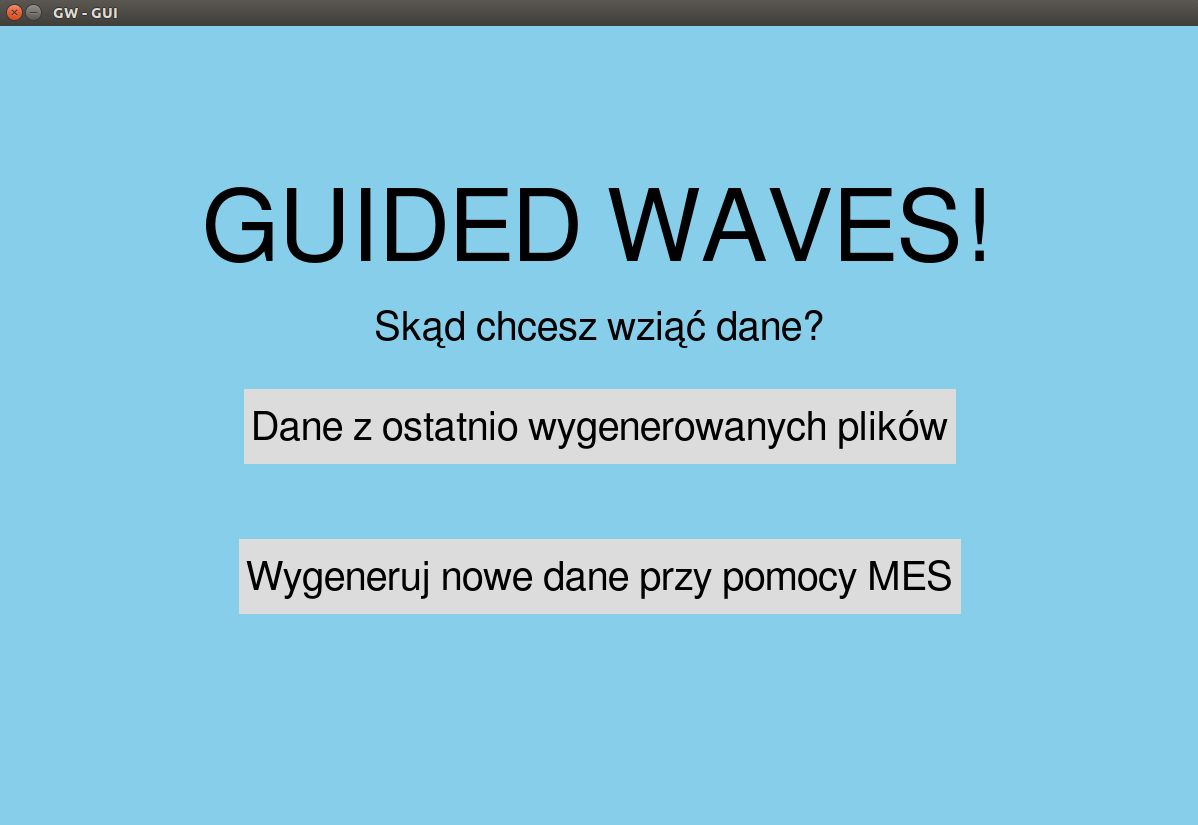
\includegraphics[width=13cm]{Zdjecia/5/kasia/gui1}
\caption{Wybór źródła danych do symulacji}
\label{fig:gui1}
\end{figure}

Po pierwsze użytkownik proszony jest o wybranie, czy chce korzystać z ostatnio wygenerowanych danych czy chce wygenerować nowe dane do symulacji. Nowe dane można również wygenerować później w dowolnym momencie. Po wybraniu opcji "Dane z ostatnio wygenerowanych plików" wyświetlany zostaje komunikat informujący o ładowaniu danych do praogramu (Rysunek \ref{fig:gui2})

\begin{figure}[h]
\centering
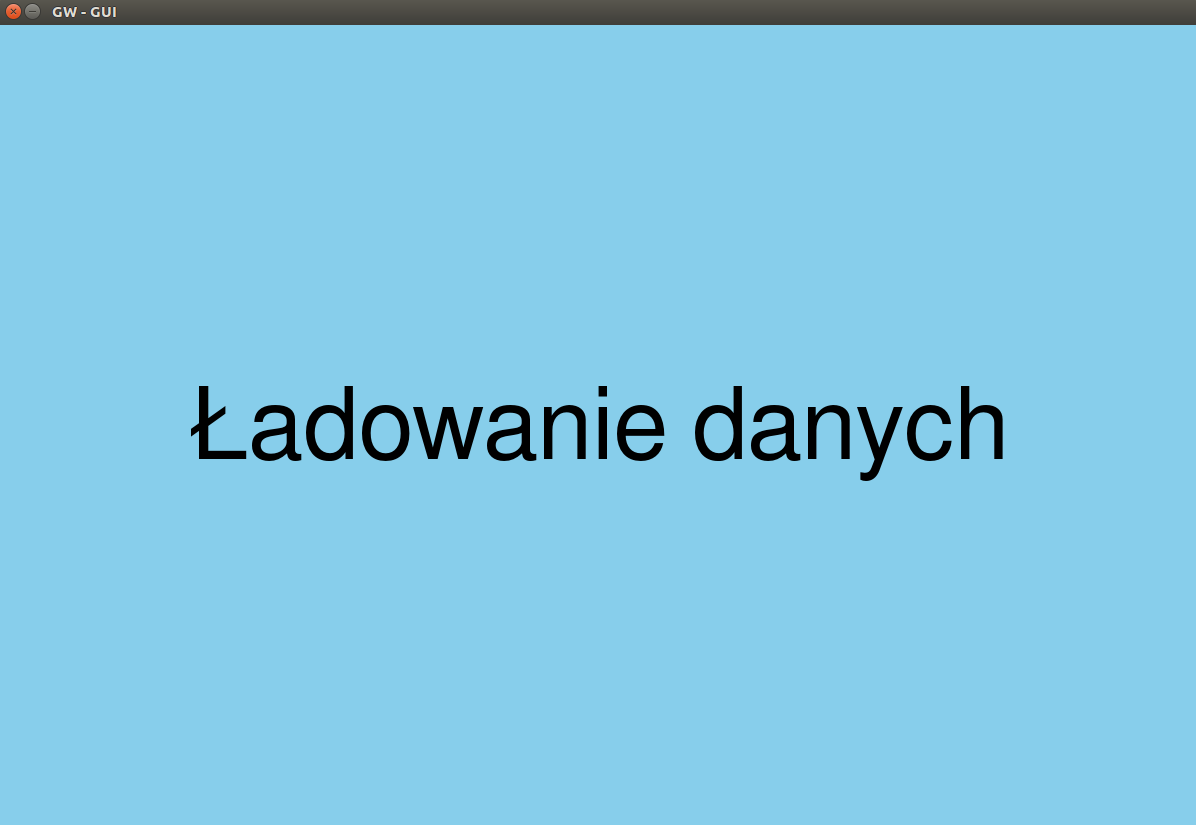
\includegraphics[width=13cm]{Zdjecia/5/kasia/gui2}
\caption{Ekran ładowania danych}
\label{fig:gui2}
\end{figure}

W tym momencie, wygenerowane przez solver dane są wczytywane do programu. A krzywe dyspersji agregowane do odpowiednich obiektów tak jak zostało to opisane w poprzednim podrzdziale. Kiedy ładowanie zostanie zakończone wyswietlany zostaje napis "Krzywe dyspersji" oraz wyświetlane są wczytane krzywe. Przedstawia to rysunek \ref{fig:gui3} \ref{fig:gui4} 

\begin{figure}[h]
\centering
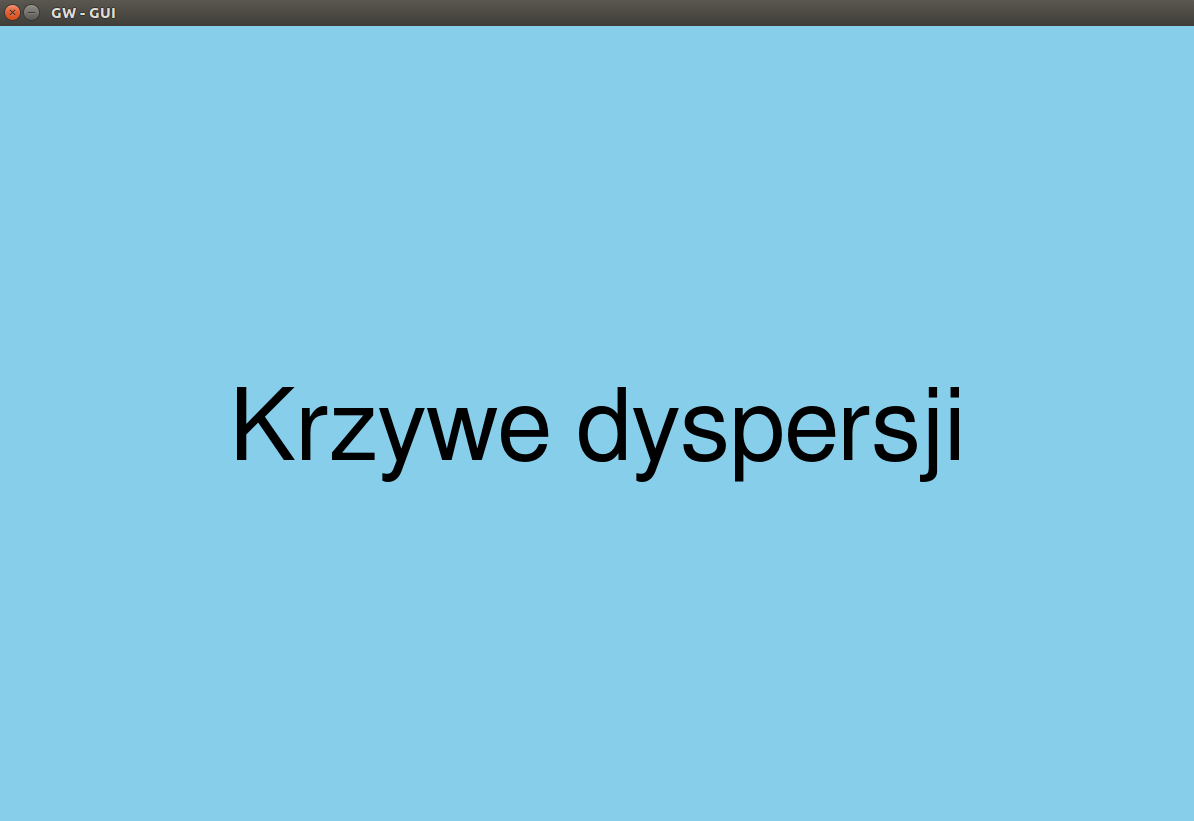
\includegraphics[width=13cm]{Zdjecia/5/kasia/gui3}
\caption{Krzywe dyspersji}
\label{fig:gui3}
\end{figure}

\begin{figure}[h]
\centering
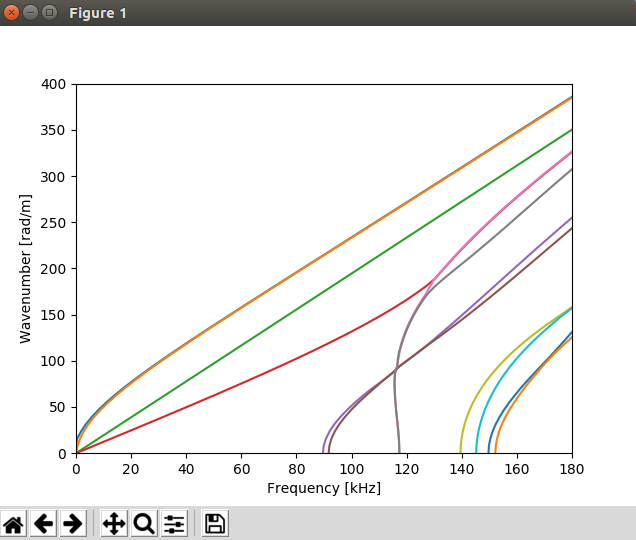
\includegraphics[width=13cm]{Zdjecia/5/kasia/gui4}
\caption{Krzywe dyspersji}
\label{fig:gui4}
\end{figure}

Aby przejść dalej należy zamknać okienko przedstawiające krzywe dyspersji. Następnie wyświetlane jest główne menu interfejsu. Przedstawia je rysunek \ref{fig:gui6}

\begin{figure}[h]
\centering
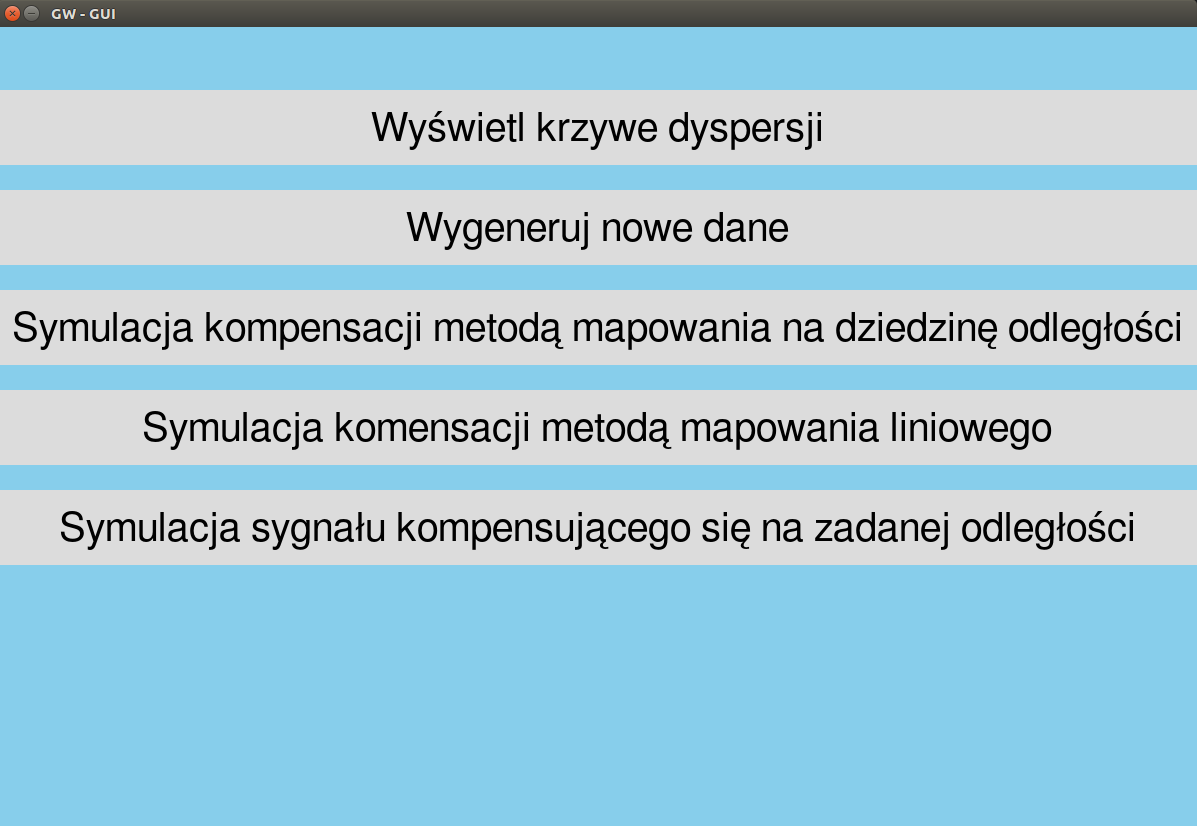
\includegraphics[width=13cm]{Zdjecia/5/kasia/gui6}
\caption{Główne menu programu}
\label{fig:gui6}
\end{figure}

W tej części do wyboru jest pięć opcji. Pierwsza z nich wyświetla okno z krzywymi dyspersji z rysunku \ref{fig:gui4}. Opcja "Wygeneruj nowe dane" przenosi użytkownika do okna z rysunku \ref{fig:gui7}. Okno to zostanie również wyświetlone po wybraniu z okna przedstawionego na rysunku \ref{fig:gui1} opcji "Wygeneruj nowe dane"

\begin{figure}[h]
\centering
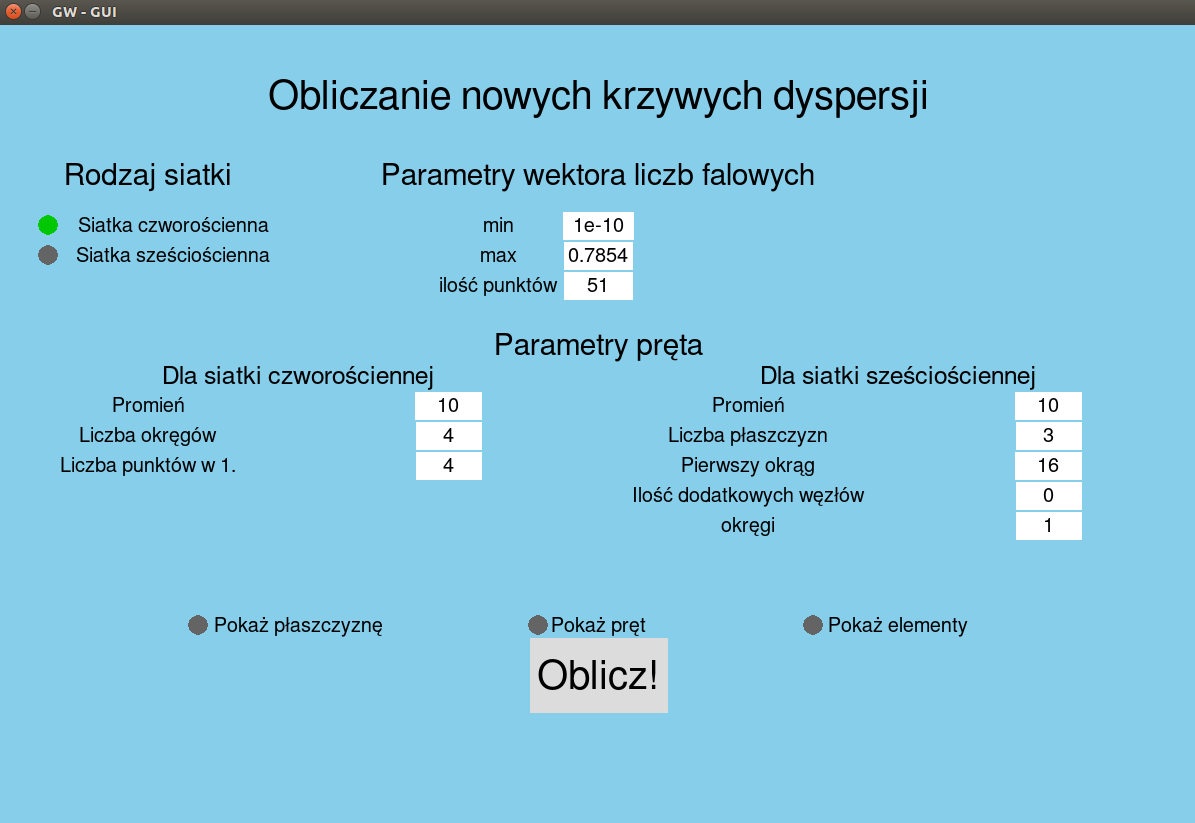
\includegraphics[width=13cm]{Zdjecia/5/kasia/gui7}
\caption{Ekran ustawień siatki}
\label{fig:gui7}
\end{figure}

W tym miejscu można wybrać rodzaj siatki, jaką użytkownik chce wygenerować. Ustawić wszystkie parametry oraz zaznczayć czy chce się wyświetlać benerowaną siatkę zarówno na płaszczyźnie, jak i w postaci pręta czy też elementów skończonych. Po wybraniu interesujących parametrów oraz zatwierdzeniu wyboru poprzez naciśnięcie przycisku "Oblicz" Pojawia się ekran informujący, że obliczenia trwają. Przedstawia to rysunek \ref{fig:gui8}
Ważną kwestią podczas wpisywania parametrów jest podawanie liczb tylko przy pomocy klawiszy znajdujących się nad klawiaturą. Klawiatura numeryczna nie jest obsługiwana, a jej użycie może spowodować błąd oraz zakończenie działania programu. Znacznik szary oznacza, iż dana opcja jest nieaktywna, natomiast znacznik zielony oznacza akywną opcję.

\begin{figure}[h]
\centering
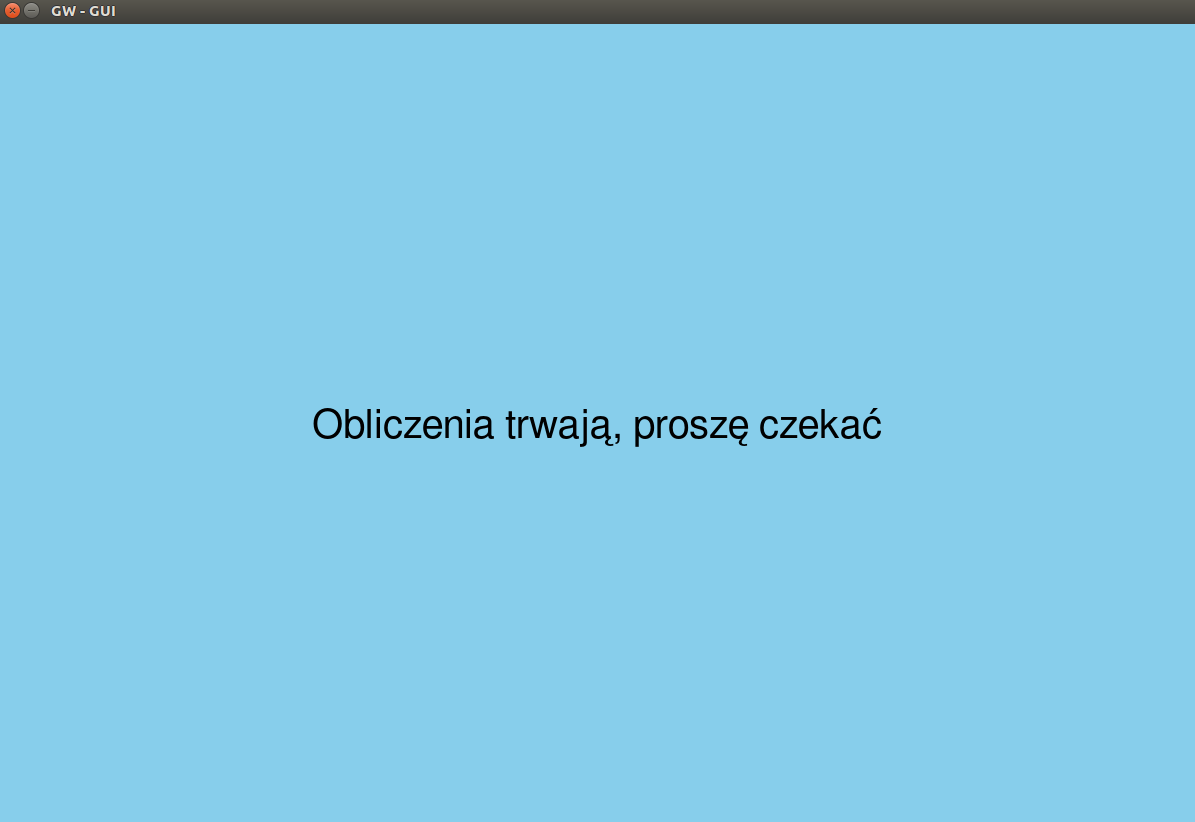
\includegraphics[width=13cm]{Zdjecia/5/kasia/gui8}
\caption{okno programu informujące o trwających obliczeniach}
\label{fig:gui8}
\end{figure}

Gdy siatka zostanie już wygenerowana program wraca do głównego menu z rysunku \ref{fig:gui6}. Kolejne trzy dostępne opcje odpowiadają opisanym już metodom kompensacji dyspersji. W całym interfejsie sygnałem propagującym orz będącym kompensowanym jest sygnał linear chirp pomnożonym przez okno Hanninga z rysunku 4.8. Po wybraniu opcji "Symulacja kompensacji metodą mapowania na dziedzinę odległości pojawia się okno z rysunku \ref{fig:guiKomp1}

\begin{figure}[h]
\centering
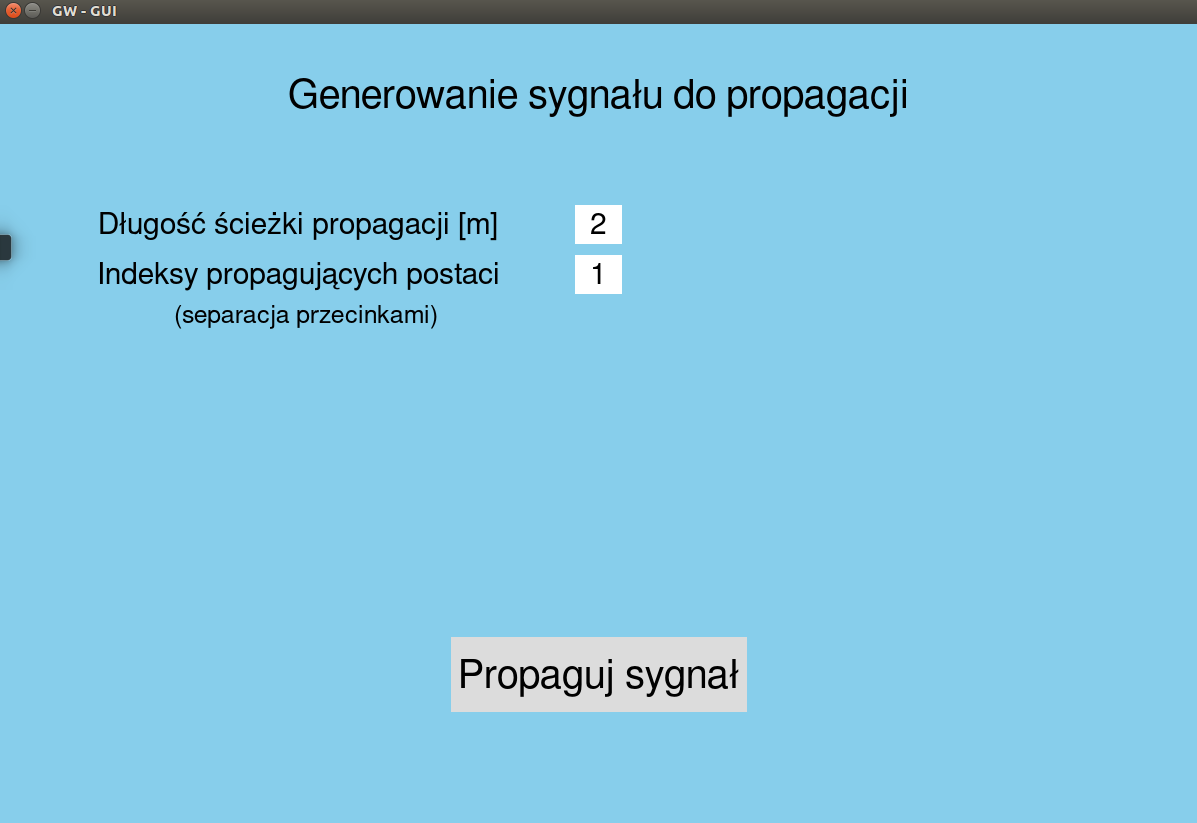
\includegraphics[width=13cm]{Zdjecia/5/kasia/guiKomp1}
\caption{okno programu informujące o trwających obliczeniach}
\label{fig:guiKomp1}
\end{figure}

W tym momencie użytkownik wybiera sygnał, jaki chce wygenerować do symulacji. Zostanie on następnie skompensowany wybraną metodą. Gdy wygenerowany sygnał zostanie skompensowany jest on wyświetlany. Po zamknięciu okienka z wyświetlonymi wynikami, program wraca do głównego menu. Po wybraniu opcji "Symulacja kompensacji metodą mapowania liniowego" program realizuje algorytm analogiczny do właśnie opisanego. Jedyna różnica to metoda jaką kompensowany jest sygnał. Wybranie opcji "Symulacja sygnału kompensującego się na zadanej odległości" otwiera okno przedstawione na rysunku \ref{fig:guiLast}

\begin{figure}[h]
\centering
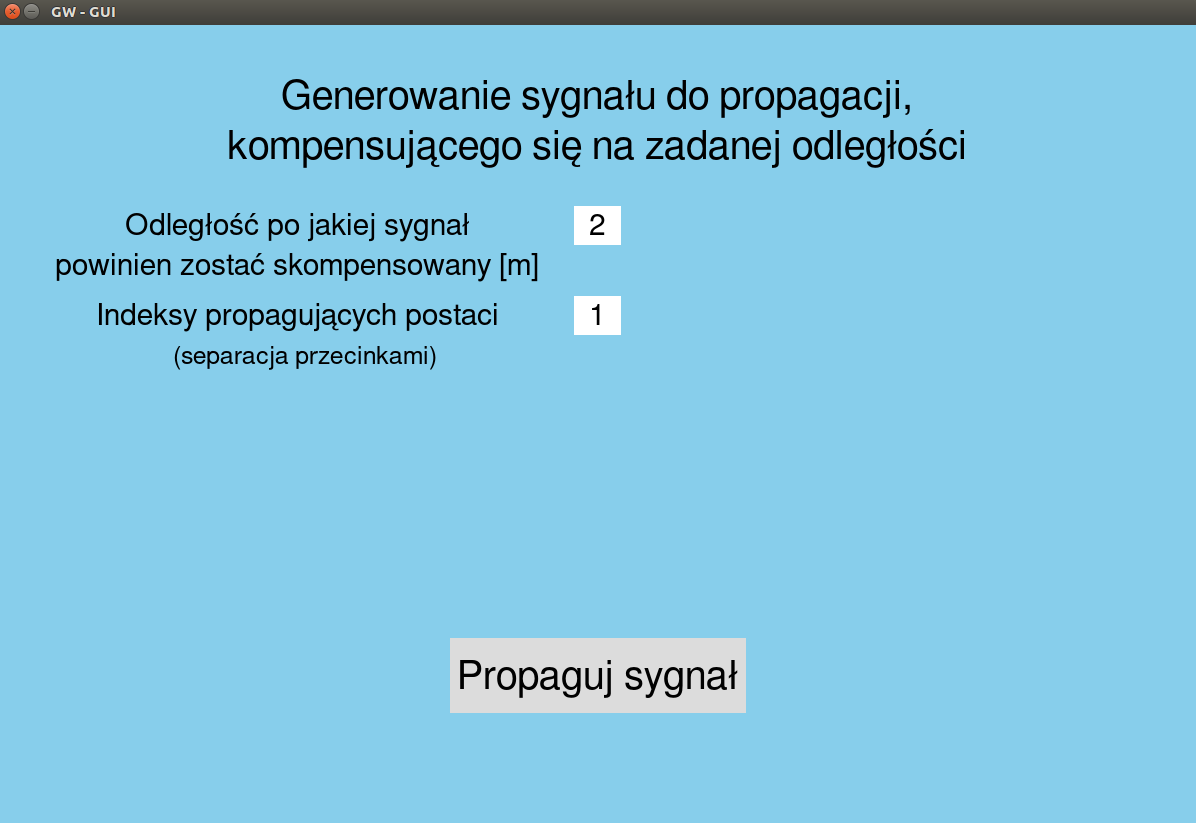
\includegraphics[width=13cm]{Zdjecia/5/kasia/guiLast}
\caption{okno programu informujące o trwających obliczeniach}
\label{fig:guiLast}
\end{figure}

Po wpisaniu odpowiednich parametrów oraz wykonaniu stosownych obliczeń wyświetlany jest wygenerowany sygnał. Po zamknięciu okna wyświetlającego wyniki pojawia się  okno pozwalające na ustawienie danych propagacji, tak aby można było zaobserwować zachowanie wygenerowanego sygnału po propagacji (rys. \ref{fig:guiLast2})

\begin{figure}[h]
\centering
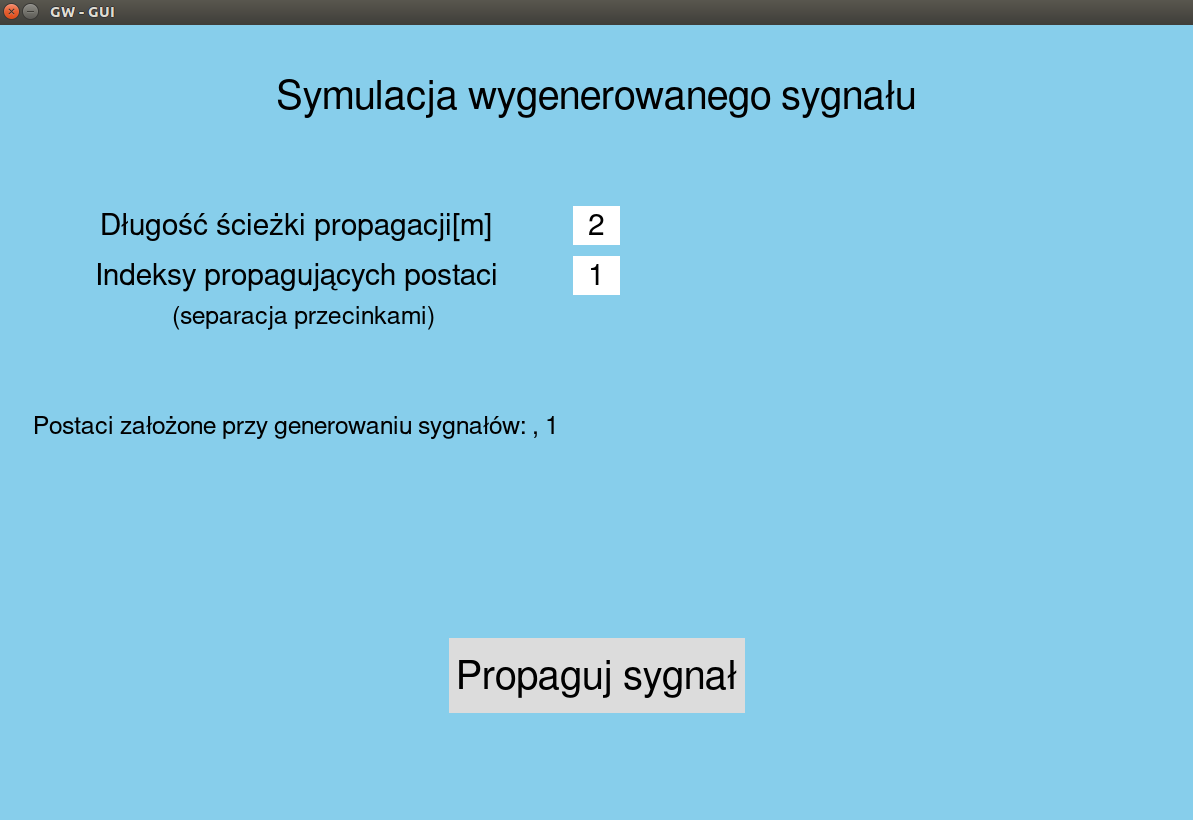
\includegraphics[width=13cm]{Zdjecia/5/kasia/guiLast2}
\caption{okno programu informujące o trwających obliczeniach}
\label{fig:guiLast2}
\end{figure}

Po skończonych obliczeniach wyświetlany jest otrzymany sygnał.

\subsection{Przykład zastosowania do wygenerowania danych dla zadanego pręta}

W niniejszej sekcji został zaprezentowany proces generowania danych dla pręta ze stali czarnej o średnicy 25 mm oraz długości 2m. Przed uruchominiem programu należy w pliku $config.py$, znajdującym się w folderze $MES\_dir$ ustawić dane materiału pręta, którego chcemy symulować. Konieczne jest podanie wartości modułu Younga, gęstości oraz współczynnika Poissona. Należy te wartości przypisać do odpowiednich zmiennych w pliku. Są to kolejno: $young\_mod$, $density$, $poisson\_coef$ Gdy odpowiednie wartości zostaną ustawione należy uruchomić program $api\_main.py$ w menu przedstawionym na rysunku \ref{fig:gui1} należy nacisnąć przycisk ,, Wygeneruj nowe dane przy pomocy mes ''. Wyświetlone zostanie okno ustawień siatki MES generowanej przez program. W tym miejscu  ustawiana zostaje średnica pręta, dla którego ma zostać wygenerowany model. Przyjmowaną jednostką jest milimetr, dlatego w polu średnica nalezy wpisać wartość 25 \ref{fig:srednica25}.

\begin{figure}[h]
\centering
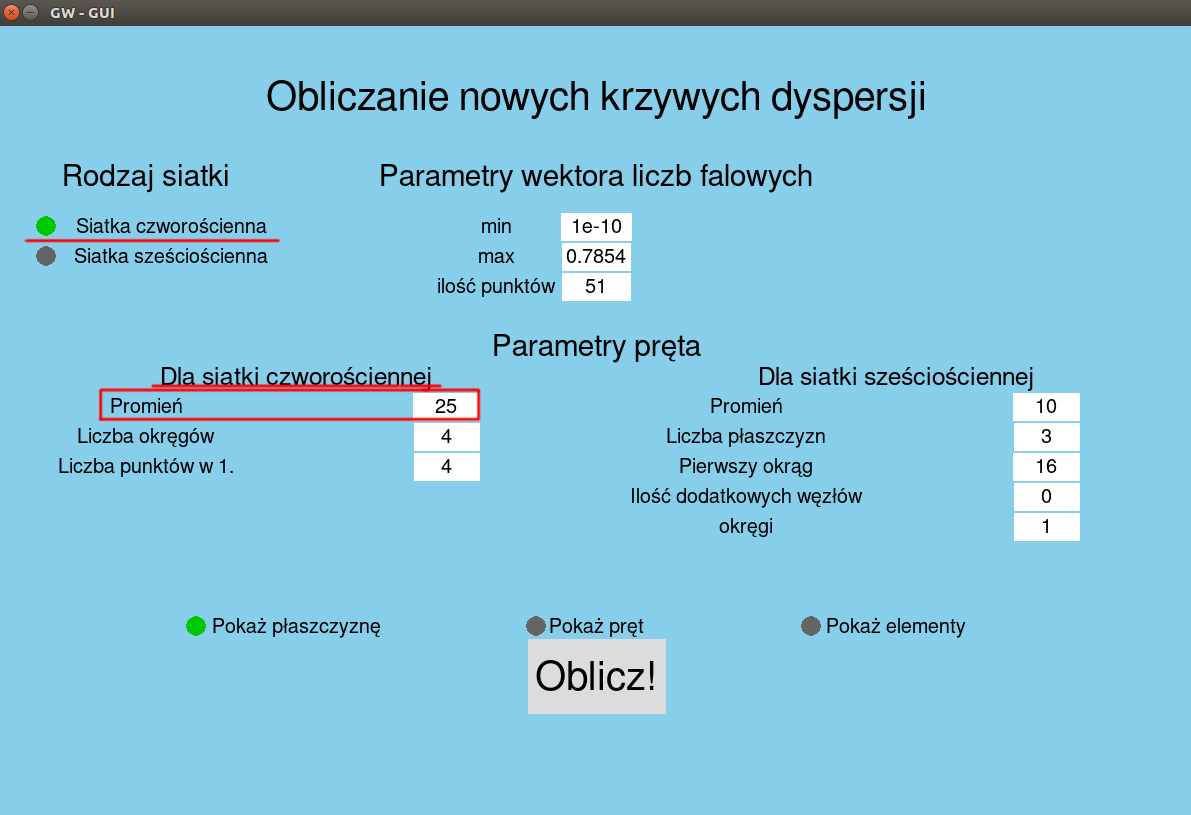
\includegraphics[width=13cm]{Zdjecia/5/kasia/srednica25}
\caption{okno programu do ustawień siatki MES}
\label{fig:srednica25}
\end{figure}

Warto zaznaczyć, iż jeśli wybrana została siatka czworościenna nalezy ustawić jedynie parametry w sekcji ,, Dla siatki czworościennej''. Parametry z drugiej sekcji nie będą brane pod uwagę. W przypadku wyboru siatki szesciościennej sytuacja jest analogiczna. Na rysunku \ref{fig:srednica25} zaznaczona została opcja ,, Pokaż płaszczyznę '' spowoduje ona, iż w trakcie trwania obliczeń, z momencie gdy zostanie wygenerowana płaszczyzna, zostanie one również wyśietlona do podglądu użytkownikowi. Przedstawia to rysunek \ref{fig:plaszczyzna}. Gdyby zostały zaznaczone również dwie pozostałe opcje, wówczas kolejno zostałyby również wyświetlone: model pręta stworzony z wygenerowanych punktów oraz model pręta z narysowaną siatką elementów skończonych. Aby rozpocząć obliczenia nalezy wcisnąć przycisk ,, Oblicz ''.

\begin{figure}[h]
\centering
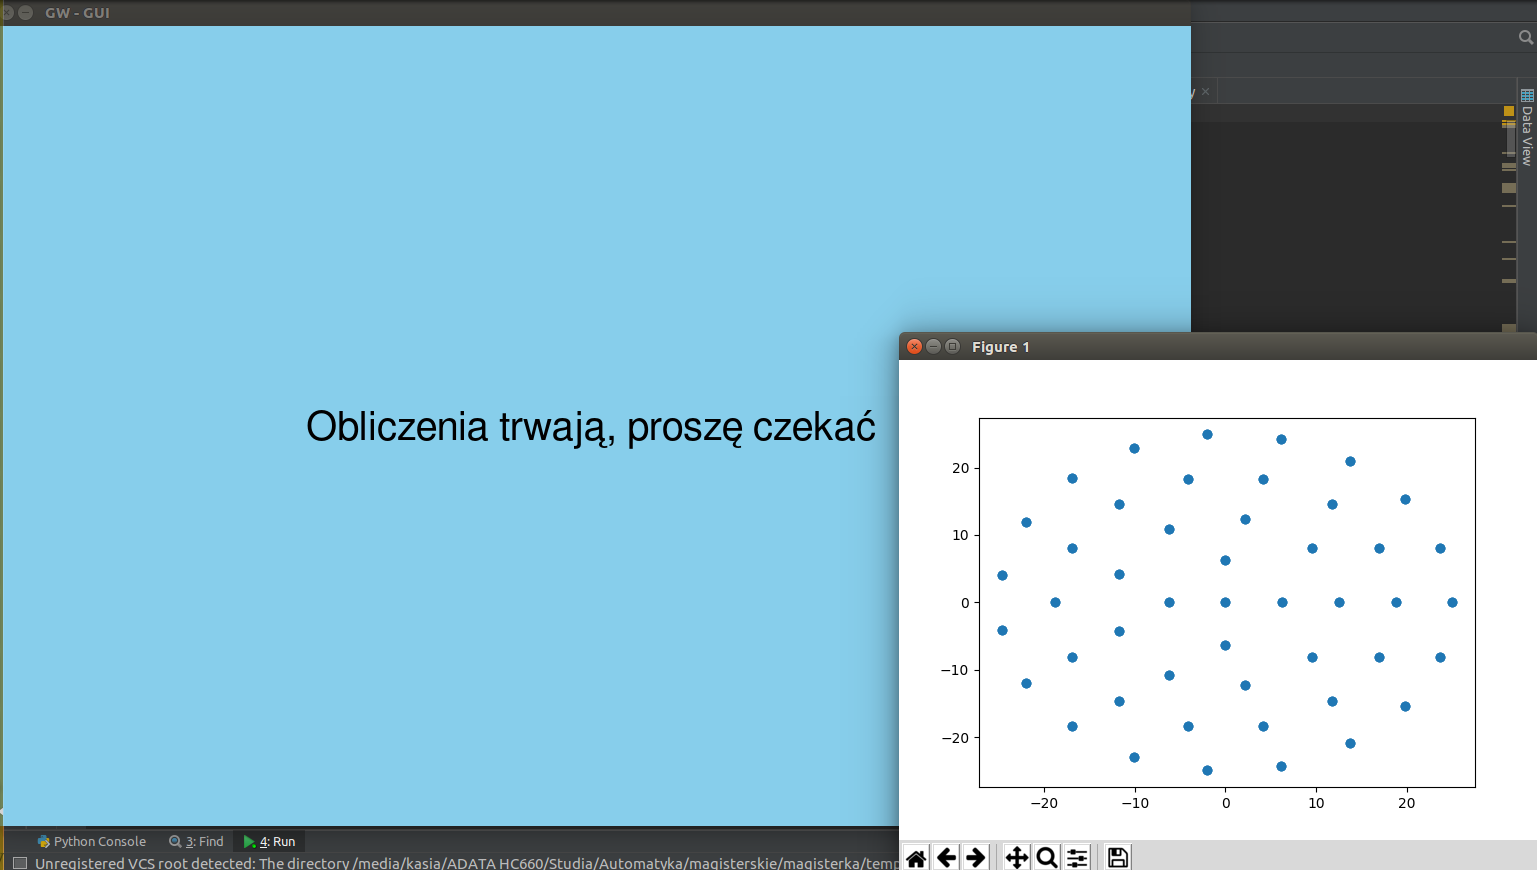
\includegraphics[width=13cm]{Zdjecia/5/kasia/plaszczyzna}
\caption{Okno obliczeń, z wyświetloną wygenerowaną płaszczyzną}
\label{fig:srednica25}
\end{figure}

Ważne jest aby po oględzinach uzyskanych wyników zamknąć każde dodatkowo pojawiające się okno, przedstawiające siatkę, pręt lub też pręt z elementami skończonymi, ponieważ bez tego program nie przejdzie do kolejnego okna. Gdy obliczenia zostaną zakończona pojawi się okno przedstawione na rysunku \ref{fig:gui6} W tym momencie nowe dane zostały wygenerowane i są przechowywane w pamięci programu. Możliwy jest teraz podgląd wygenerowanych krzywych dyspersji poprzez przycisk '' Wyświetl krzywe dyspersji''. Przedstawione zostało to na rysunku \ref{fig:krzywesa}.

\begin{figure}[h]
\centering
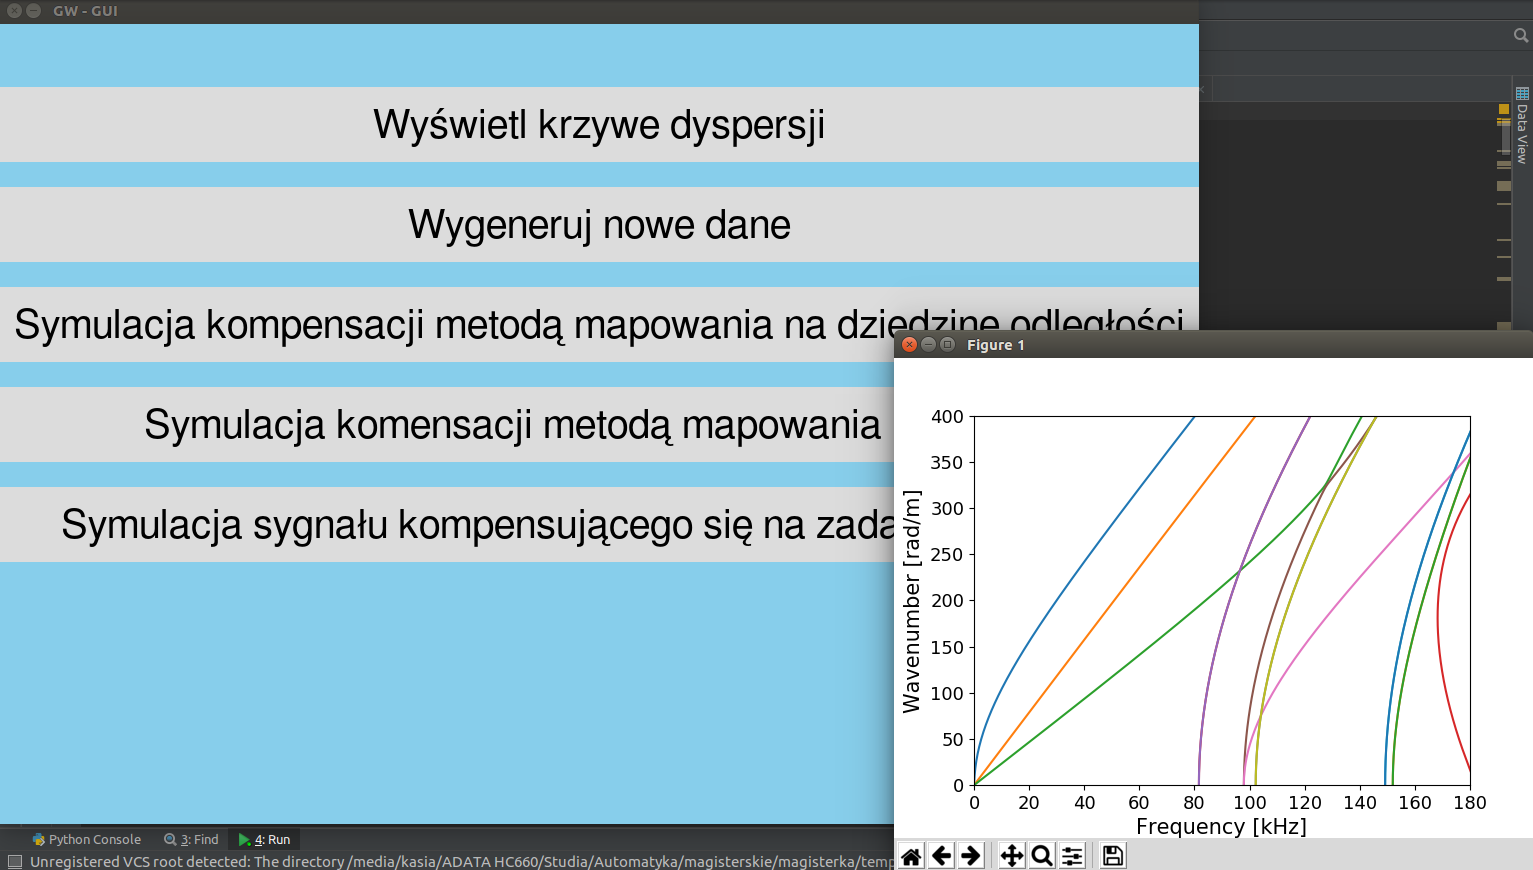
\includegraphics[width=13cm]{Zdjecia/5/kasia/krzywesa}
\caption{Okno programu z wyswietlonymi krzywymi dyspersji}
\label{fig:krzywesa}
\end{figure}

Aby móc korzystać z pozostałych funkcji programu należy zamknąć okienko z krzywymi.

Na tak wygenerowanych danych można testować zaimplementowane metody kompensacji dyspersji. Na przykład metodę mapowania sygnału z dziedziny czasu na dziedzinę odległości. Aby to zrobić należy nacisnąć przycisk ,,Symulacja kompensacji metodą mapowania z dziedziny czasu na dziedzinę odległości. Następnie wyświetlony zostanie ekran służący do generowania sygnału omówionego na początku rozdziału 4., który przepropagował zadaną odległość. Aby zasymulować sygnał, został wprowadzony do założonego na początku sekcji pręta, przepropagował jego długość, wynoszącą 2 metry i został odebrany na jego końcu, jako długość ścieżki propagacji należy wpisać 2. Natomiast indeksy propagujących zostały przyjęte jako pierwsze trzy postaci. Powyższe ustawienia ilustruje rysunek \ref{fig:genersygnal}

\begin{figure}[h]
\centering
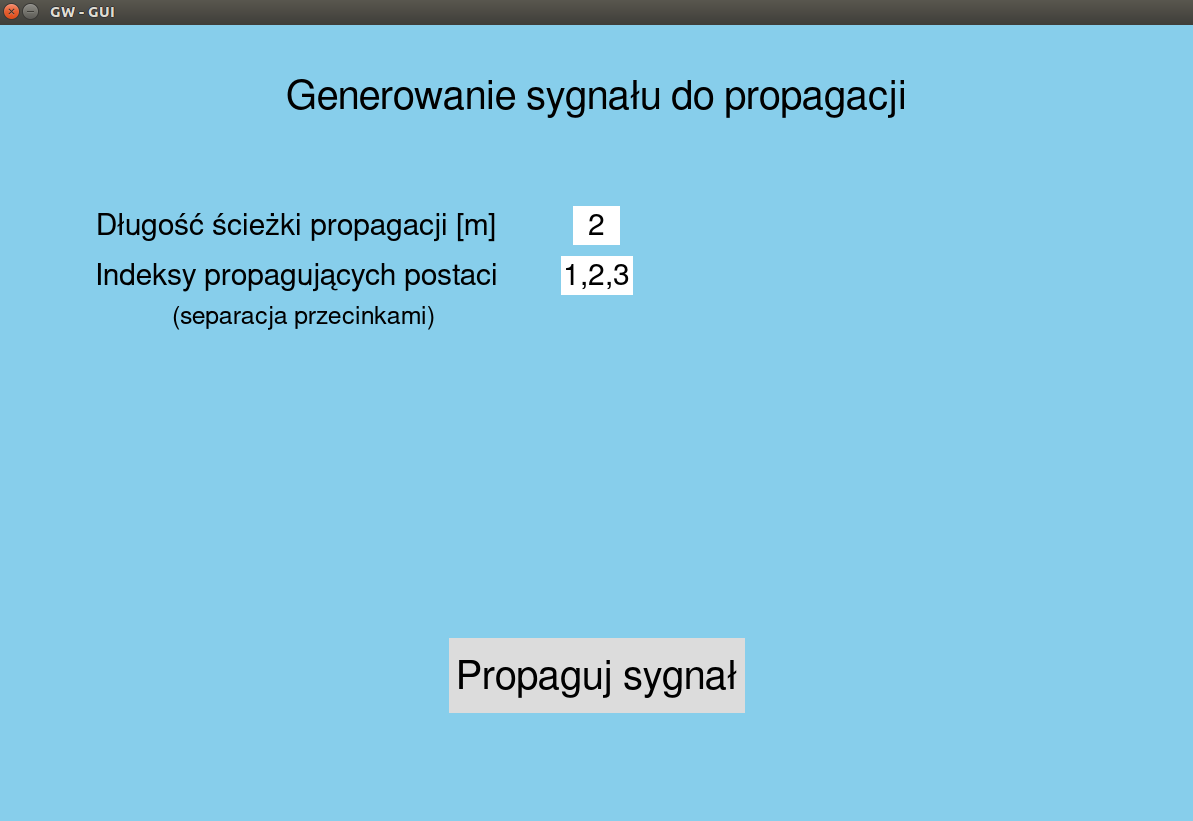
\includegraphics[width=13cm]{Zdjecia/5/kasia/genersygnal}
\caption{Okno programu przedstawiające ustawienia generowanego sygnału}
\label{fig:genersygnal}
\end{figure}

Gdy obliczenia zostaną zakończone, wyświetlone zostanie okno z wynikami kompensacji. Po jego zamknięciu znów pojawi się główne menu, z którego poziomu możliwa jest symulacja kompensacji opracowanymi metodami, wyświetlenie aktualnie używanych krzywych dyspersji oraz wygenerowanie nowych danych.
